\documentclass[11pt]{book}
\usepackage[usenames,dvips,pdftex]{color}
\usepackage[pdftex]{color,graphicx}
\usepackage{hyperref}
\usepackage{array}
\usepackage{tabularx}
\usepackage{overpic, epic}
\usepackage{float}
\usepackage{textcomp}
\usepackage{wrapfig}

\hypersetup{colorlinks=true, filecolor=black, linkcolor=black, urlcolor=blue, citecolor=black}


\graphicspath{{./images/}}

\begin{document}
\title{PR2 user manual}
\author{Willow Garage}
\newcommand{\TODO}[1]{\textcolor{red}{TODO: #1}}
\maketitle
\newpage
\tableofcontents
\newpage
\chapter {Introduction}
This manual is intended to give you enough information to successfully install, use, and develop code on your PR2 robot.  The software on the PR2 is provided by software based on ROS.  The recommended source of information for learning about ROS and the higher-level software available for the PR2 is http://ros.org

If you want to get started running the PR2 as quickly as possible, please start with Chapter 2 on safety (seriously - the PR2 is a big machine and can cause serious injuries or death), and then you can skip to chapter 5 to learn how to start up and run the PR2.

\section{Before you start}
\paragraph{Space} To use PR2 you will need to have enough room for it to drive around and move it's arms.  The PR2 is designed to move through ADA-compliant spaces (Americans with Disabilities Act), so corridors should be at least 36" wide, doorways should be at least 32", and the ground should be flat and level.  You will need enough space for the PR2 to move around and perform tasks.
\paragraph{Safe Environment} The space where the PR2 operates should be free of hazards.  Specifically, stairways or other fall hazards can pose an extreme danger and the PR2 should not be operated near any type of dropoff.  You should also avoid hazardous objects, such as knives, sources of fire, hazardous chemicals, or furniture that could be knocked over.  See chapter 2 for more details on making sure your environment is safe.
\paragraph{Electrical} The PR2 recharges using a standard 120V American power outlet.  The robot can draw 15A of current when plugged in, so we strongly recommend recharging the PR2 only on outlets with no other devices on the circuit breaker.
\paragraph{Development tools}
You will need at least one laptop or desktop computer to use to connect to the robot.  The PR2 ships with a base-station computer, which is a desktop, but you will need to provide a screen, mouse, and keyboard.  A laptop with wireless access is ideal.
\paragraph{Linux} We highly recommend familiarity with the Linux command-line.  The PR2 computers both run Ubuntu, and since they don't have attached displays, all tasks on them have to be performed by logging in remotely (e.g. via ssh).
\paragraph{ROS} Since all the PR2 software is based on ROS, running through the beginning tutorials available at ROS.org will help you understand the structure of the software on the robot and will give you tools to understand the software that's running and the data that is moving around in the system.
\paragraph{PR2 Safety} Be sure to familiarize yourself with the contents of the following chapter on safety before using the PR2.


\chapter{Safety}

Safety is a key goal at Willow Garage.  It is important, it is challenging, and it is a continual process shared by the designer, user, and administrator of a robot.  In the following we provide an overview of the issues, describe some safety-related design features, enumerate a set of basic usage guidelines to support safety, and finally detail the explicit safety program.

\section{Overview}

Safety is a vitally important concern whenever you are around a PR2. It is a heavy piece of equipment with many moving parts. It travels though the environment and can carry and manipulate a wide variety of objects. Its movements and actions are not completely predictable. It can cause significant damage if it falls on or runs over someone. There are several ways it can pinch, grab, and twist fingers or other parts of the body. It can wield dangerous implements and knock heavy things over. You must always be cautious and attentive when you are around a PR2.

Safety is neither absolute criterion nor a one-time event.  Instead it is an appreciation that risks are inherent to any robotic endeavor and they must be minimized as well as weighed against benefits.  It is a goal for which the entire community must continually strive.

We emphasize safety to avoid harm to any person, animal, or equipment.  We also recognize that robots in general will not gain wide acceptance or fulfill their potential unless the community can adequately manage safety.

Managing safety is challenge when dealing with any complex engineering system.  In the case of the PR2, consider also the open, extensible, programmable, experimental nature of the platform.  The PR2's capabilities and behaviors change over time, with user interactions, and with re-programming.

With this in mind, Willow Garage has chosen a three-fold approach.  First, we have designed the PR2 to minimize potential risks and maximize inherent safety, cognizant of its uncertain uses.  Second, we communicate to all users about how to minimize risk. And third, we have implemented an explicit safety program to ensure that the community continues to identify potential hazards, seek design mitigations, and communicate effective usage guidelines.

\section{Design Features}

We have designed both hardware and software to minimize risks, while retaining the power of an open platform.  These aspects of the design are often described as inherent safety features.  For example, PR2's arms are back-drivable.  That means when an arm encounters an object, be it a table or a person, the interaction will drive the motors back and bring the arm to a stop.  The PR2 arms can't "punch through" an object the way traditional industrial robots can.

We have further designed the PR2 arms with relatively small motors with respect to their payload.  This is possible due to a spring counterbalance offsetting the gravity forces acting on the arms.  That is, the arms do not need to hold their own weight against gravity.  And so the motors need only be strong enough to hold the payload.  The arms simply can't push very hard.

In software, we have incorporated low level checking to limit the current in a motor, to limit the velocity of a motor, and to limit the range through which a motor should travel.  We obviously discourage users and developers from changing these configurations.  High level applications also avoid obstacles in navigation and movement using the various on-board sensors.

These design choices also help make PR2 robust.  However, a robot with the PR2's capabilities can never be absolutely safe. Your safety as well as the safety of others critically depends on your constant attention. You must be aware of the potential dangers, anticipate possible problems, and plan to prevent their occurrence.

\section{General Usage Guidelines}

While many guidelines for the safe use of a robot stem from common sense, we enumerate a basic set here.  We stress the importance of following these guidelines but re-emphasize that these guidelines alone do not guarantee safety but reduce risk.
\begin{itemize}
\item Every organization that uses a PR2 must appoint a Safety Officer.
\begin{itemize}
\item The Safety Officer's contact information should be known by everyone in the organization who uses the PR2 (including designers, developers, programmers, and end-users).
\item Further details of the Safety Officer's roles and responsibilities are described in section 2.4.
\end{itemize}
\item Before operating or working with the PR2 you must do the following:
\begin{itemize}
\item view the safety video
\item read this User Manual, particularly Chapter 2 on Safety
\item read and understand the latest list of potential hazards
\item know how to contact your organization's Safety Officer
\end{itemize}
\item Supervise children, visitors, and anyone who has not followed the previous guideline.  In particular, make sure they
\begin{itemize}
\item do not come within range of the PR2 when active
\item are aware the robot could move unexpectedly and is potentially dangerous
\item are not alone with the PR2
\item do not operate the PR2
\end{itemize}
\item Maintain a safe environment.  Safety is not only an issue of how you operate the robot, but also the environment.
\begin{itemize}
\item Make sure the robot has adequate and level space for any expected or unexpected operation
\item Make sure the the environment is free of objects that could pose a risk if knocked, hit, or otherwise affected by the PR2
\item Make sure no animals are the near the robot.
\end{itemize}
\item The PR2 is designed to operate in an laboratory environment
\begin{itemize}
\item It should not be operated outdoors
\item It should not come in contact with liquids
\item It should not be operated within 7 meters of the top of a stairway
\end{itemize}
\item Anticipate potential problems and hazards.  Always imagine what might happen if the robot malfunctions or behaves in a way different from the desired action.  Be vigilant.
\item The operator should always have immediate access to the run/stop and stop the robot at the first sign of a problem.
\item Use common sense when operating the robot.
\begin{itemize}
\item Do not allow the robot to grab or hit any person
\item Do not allow the robot to drive into contact with or over any body part.
\item Do not allow the robot to interact with any sharp or dangerous items
\end{itemize}
\item Pay attention to warning labels on the robot.
\item Do not remove the covers of a PR2 without prior and appropriate instruction by Willow Garage. There are high voltages and a variety of pinching and other mechanical dangers in the interior of the robot.
\item Do not modify or remove any part of the software safety features.
\end{itemize}

\section{Safety Program}

Safety is a continual process, and in particular should include

\begin{itemize}
\item an awareness of risks
\item a critical examination to expose risks, assess risks, discover mitigations, and evaluate trade-offs
\item any deliberate actions needed to minimize and mitigate current and future risks.
\end{itemize}

To facilitate this process and communication within the community, Willow Garage has implemented a safety program.

\subsection{Willow Garage Safety Board}

The Willow Garage Safety Board identifies hazards related to Willow Garage products and ensures that appropriate actions are taken to mitigate those hazards. The Board maintains a database to keep track of the hazards and mitigation actions. To identify additional hazards for the database, the Board commissions Hazard Brainstorming Meetings and reviews incident reports from the field. To initiate actions that reduce the severity and/or likelihood of specific hazards, the Board commissions Hazard Response Projects. To ensure that appropriate actions remain in force, the Board commissions Hazard Response Audits. The Board works with Safety Officers in external organizations to improve safety across all users of Willow Garage products.
The core Safety Board includes senior members of the Willow Garage management. Additional employees serve for term appointments. Members of the Board spend at least one day a month on safety related work.
\subsection{Hazard Database}

The Hazard Database includes three types of entity: Hazards, Incidents, and Responses.
Hazards describe things the system might do that can cause damage, for example, running into something or falling down stairs. Each Hazard includes an estimate of its severity and likelihood of occurrence. Based on these estimates, the Hazard is assigned a priority for action.
Incidents describe specific examples of Hazards, either things that have actually occurred or hypothetical occurrences. Each Incident is associated in the database with the Hazard(s) that it exemplifies.
Responses describe actions that reduce the severity and/or likelihood of a hazard. These can involve changes to the design or documentation of the hardware and software, additional warnings to the community, or changes to the safety training and video.

The information in the Hazard Database is summarized in several reports that document the current understanding of potential hazards and the associated mitigating actions. Chief among these is the Prioritized Hazard Report, which lists the Hazards in the database in order of their priority.

\subsection{Safety Officers}

Each organization that uses Willow Garage products will appoint a Safety Officer who is responsible for all aspects of safety in the use of those products. The Safety Officer will:
\begin{itemize}
\item remain informed of all known safety hazards and mitigations,
\item ensure that all known mitigations are implemented in their organization,
\item ensure that everyone involved with the products receives safety training,
\item report any safety incidents to Willow Garage in a timely fashion, and
\item work with the Willow Garage Safety Board to improve safety.
\end{itemize}

\chapter{Safety and the PR2}
Point out which parts of the code are considered part of the hardware safety systems (e.g. joint current limits), and make it clear that changing them can cause problems.

Talk about guidelines for safe operation (e.g. is it OK in a normal lab environment?)

\chapter{PR2 hardware}

\section{What's in the box}
The PR2 will arrives in a big crate.  In the crate should be:
\subsection{PR2 robot}
\subsection{Wireless run-stop}
\label{wirelessrunstop}
The PR2 comes with an \href{http://www.omnexcontrols.com/products/portable/t50.html}{OMNEX T50} 
wireless run stop transmitter which when stopped or out of range will halt the motors and put the power system in standby mode. 

\begin{figure}[h]
\centering
\includegraphics[width=150px]{run_stop.png}
\caption{The PR2 wireless run stop.}
\label{fig:runstop}
\end{figure}

To start the run stop transmitting, press the green start button (Figure~\ref{fig:runstop}) which will start the transmitting 
light flashing. While transmitting the run stop has a range of approximately 800ft. The run stop is powered by 4AA batteries 
when the batteries are low the battery light will flash warning you to change the batteries.

\subsection{Wireless Joystick}
The PR2 ships with a bluetooth joystick for teleoperating the robot. The bluetooth joystick is a 
\href{http://www.sonystyle.com/webapp/wcs/stores/servlet/ProductDisplay?catalogId=10551&storeId=10151&langId=-1&productId=8198552921665411965#additionalImage1%22}{Sony DUALSHOCK®3} 
wireless controller and can be charged using any standard USB A to mini-B USB cable. For more information please see the 
\href{http://www.ros.org/wiki/ps3joy}{ps3joy} package at \href{http://www.ros.org}{ros.org}.

\subsection{Base-station computer}
\section{Mechanism}
PR2 is a 32-dof mobile manipulator with a mobile base, two arms, and a variety of sensors on a pan-tilt head.
\subsection{Robot anatomy}
Include the information from the robot anatomy document here.  Official names of all components, links, and joints in the robot with pictures.
\subsection{Drivetrains}
Discuss the drive-train approach, how/why things work, what types of errors we expect to see and don't expect to see
\subsection{Motion control}
Describe motion control architecture, capabilities, performance.
\subsection{Mechanical specs}
\subsubsection{Environmental specs}
\subsubsection{Forces and torques}
\subsubsection{Joint limits and range of travel}

\section{Sensors}
The PR2 has a variety of sensors spread out over it's body:
\subsection{Base Laser}
The base laser of the PR2 is \href{http://www.hokuyo-aut.jp/02sensor/07scanner/utm_30lx.html}{Hokuyo Top-URG (UTM-30LX)} 
scanning range finder that has a 30m and 270$^\circ$ scanning range. For more information please see the 
\href{http://www.ros.org/wiki/hokuyo_node}{hokuyo\_node} package at \href{http://www.ros.org}{ros.org}.

\subsection{Tilting Laser}
In addition to the base laser, the PR2 has a \href{http://www.hokuyo-aut.jp/02sensor/07scanner/utm_30lx.html}{Hokuyo Top-URG (UTM-30LX)}
mounted on a tilting platform below the pan-tilt head. The tilting platform can sweep the scanning 
laser through 135$^\circ$ ($+90^\circ$ and $-45^\circ$ from level) and can be controlled using the
default laser\_tilt\_controller. For more information please see the \href{http://www.ros.org/wiki/hokuyo_node}{hokuyo\_node} 
and \href{http://www.ros.org/wiki/pr2_default_controllers}{pr2\_default\_controllers} packages at \href{http://www.ros.org}{ros.org}.

\subsection{Head Cameras}
The PR2 pan-tilt head has three cameras and a textured light projector:
\begin{description}

\item[Wide Stereo Camera]
The wide stereo of the PR2 is part of the dual stereo pair and is a 100Mb color ethernet camera. The wide stereo uses the
\href{http://www.aptina.com/products/image_sensors/mt9v032c12stc/#overview}{Aptina MT9V032C12STC} imager chip
and has a max resolution of 752 x 480 pixels at 15 fps. The camera has a field of view (FOV) of approximately 
$90^\circ$ and a 2.5mm F2.5 \href{http://www.mars-cam.com/lenses/ccd_cmos/Technology%20Report(V-4402.5-2.5-HR).pdf}{Marshall V-4402.5-2.5-HR} 
lens. For more information please see the \href{http://www.ros.org/wiki/wge100_camera}{TODO} package
at \href{http://www.ros.org}{ros.org}.

\item[Narrow Stereo Camera]
The narrow stereo of the PR2 is part of the dual stereo pair and is a 100Mb monchrome ethernet camera. 
The narrow stereo uses the \href{http://www.aptina.com/products/image_sensors/mt9v032c12stm/#overview}{Aptina MT9V032C12STM} 
imager chip and has a max resolution of 752 x 480 pixels at 15 fps. The camera has a FOV of approximately $55^\circ$ and 
a 5.6mm F2.0  \href{http://www.mars-cam.com/lenses/ccd_cmos/Technology%20Report(V-4405.6-2.0-HR).pdf}{Marshall V-4405.6-2.0-HR}
lens. For more information please see the \href{http://www.ros.org/wiki/wge100_camera}{TODO} package
at \href{http://www.ros.org}{ros.org}.

\item[Gigabit Ethernet Camera]
The PR2 has a gigabit ethernet camera located to the left of the dual stereo pair on the pan-tilt head. 
The gigabit ethernet camera is a \href{http://www.prosilica.com/products/gc2450.html}{Prosilica GC2450C} 
which uses the Sony ICX-625AQ imager chip and has a max resolution of 2448 x 2050 pixels at 15 fps. 
Additionally, the gigabit ethernet camera has a 8mm F1.4-F16 \href{http://www.kowascope.com/frontend/proddetail.asp?pn=LM8JC&co=10000348}{Kowa LM8JC} lens.
For more information please see the \href{http://www.ros.org/wiki/prosilica_camera}{prosilica\_camera} package
at \href{http://www.ros.org}{ros.org}.

\item[Textured Light Projector]
The PR2 has a textured light projector located to the right of the dual stereo pair on the pan-tilt head. The projector has a 
FOV of approximately $55^\circ$ and a 5.6mm F2.0 \href{http://www.kowascope.com/frontend/proddetail.asp?pn=LM12JC&co=10000348}{Kowa LM12JC} 
lens.  For more information please see the \href{http://www.ros.org/wiki/TODO}{TODO} package at \href{http://www.ros.org}{ros.org}.

\end{description}

\subsection{Forearm cameras}
Each forearm of the PR2 is equipped with a 12V 100Mb color ethernet camera. The forearm camera uses the 
\href{http://www.aptina.com/products/image_sensors/mt9v032c12stc/#overview}{Aptina MT9V032C12STC}  imager chip
and has a max resolution of 752 x 480 pixels at 15 fps. Additionally, the forearm camera has a 2.5mm F2.0 lens.  
For more information please see the \href{http://www.ros.org/wiki/wge100_camera}{wge100\_camera} package
at \href{http://www.ros.org}{ros.org}.

\subsection{Gripper Sensors}
\begin{description}

\item[Accelerometer]
The gripper of the PR2 is equipped with a \href{http://www.bosch-sensortec.com/content/language1/html/3474.htm}{Bosch BMA150} 
digital triaxal accelerometer. The measurement range ($\pm$2g, $\pm$4g, or $\pm$8g) and bandwidth (25Hz - 1500Hz) 
of the accelerometer can be selected in software. For more information please see the \href{http://www.ros.org/wiki/wge100_camera}{TODO} 
package at \href{http://www.ros.org}{ros.org}.

\item[Fingertip Pressure Sensors]


\item[Calibration LED]

\end{description}

\subsection{Inertial measurement unit}
The PR2 has an inertial measurement unit (IMU) located next to the tilting laser. The IMU is a 
\href{http://www.microstrain.com/3dm-gx2.aspx}{MicroStrain Inertial-Link 3DM-GX2} which has an 
accelerometer range of $\pm$5g and a gyro range of $300^\circ/s$. For more information please see 
the \href{http://www.ros.org/wiki/microstrain_3dmgx2_imu}{microstrain\_3dmgx2\_imu} package at \href{http://www.ros.org}{ros.org}.

\subsection{Speaker}
The PR2 has two \href{http://www.logitech.com/index.cfm/speakers_audio/home_pc_speakers/devices/199&cl=us,en}{Logitech V20 notebook speakers} 
that are located under the pan-tilt head on either side of the tilting laser. For more information please 
see the \href{http://www.ros.org/wiki/sound_play}{sound\_play} package at \href{http://www.ros.org}{ros.org}.


\section{Power system}
\subsection{Overview}
The PR2 has a Lithium-ion (Li-ion) battery system that is charged off of 120V wall current and provides power the computers, motors, and sensors in the system.  Power distribution is controlled by the {\it Power Board}, which communicates over Ethernet.
\subsection{Power Busses}
The robot has several internal power busses:
\begin{description}
\item[120v] The robot has a 3-prong IEC320 plug in the back, which is connected through a circuit breaker to the inputs of the four AC-DC converters that are used to charge the battery packs.  The system is designed to pull up to 15A, so it is OK to plug the robot in to any 15A wall socket, but you should make sure there aren't other devices which draw significant power, such as computers, on the same circuit.
\item[Motor Power Bus] The motor controllers are fed from circuit breakers on the power board that can be in one of thre states.  When enabled, they provide a direct connection to the unregulated battery power, which ranges from 52V when the batteries are fully discharged up to 72V when connected to wall power.  When the motors are in standby mode, the power board provides a low-power 18V supply which is used for communication and to maintaing encoder position counts.  In the event of a major power-system problem, or if manually disabled, these circuit-breakers will also shut completely off without cutting power to the computers or sensors.  There are three independent motor power busses - left arm, right arm, and base/head.
\item[12V system bus]
12V power for sensors.  This is also the recommended source of power for user modifications. Provided by the power board.
\item[12V computer power]
12V power for computers.  Provided by the power board.
\end{description}
\subsection{Batteries}
The battery system has four battery bays comprised of four \href{http://www.oceanserver-store.com/18.html}{Ocean Server BA95HC-FL}
14.4V Li-ion batteries, a \href{http://www.v-infinity.com/adtemplate_child.asp?c=710918&p=903285&catky=764537&subcatky1=46887&subcatky2=320934}{V-INFINITY VF-S320-18A-CF}
18V AC-DC Power Supply, and a \href{http://www.oceanserver-store.com/xpmibamamo.html}{Ocean Server XP-04SRW} four channel high current battery controller. 
This provides approximately N hours of countinous operation after a full recharge. For more information please see the 
\href{http://www.ros.org/wiki/ocean\_server}{ocean\_server} package at \href{http://www.ros.org}{ros.org}.

\subsection{Power board}

\subsection{Modularity and expansion}
Talk here about the head bolt-pattern and electrical connections, plus other interfaces.  Question of whether to try to have full specs for all interfaces or not.
\subsection{Tutorials} 
\begin{itemize}
\item{Seeing the power state in pr2\_dashboard}
\item{Turning on and off, understanding e-stop and enable/disable}
\item{Charging}
\item{What to do if PR2 doesn't turn on}
\item{Adding a new component to the system}
\end{itemize}



\chapter{PR2 Computers}
This section covers the configuration of the computers and software that comes installed on the robot
\section{Computer hardware}
The PR2 has two computers, each with 24 Gb of random-access memory (RAM), 2
quad-core Nehalem processors, and two attached hard-drives.  The
motherboards are XXX from Rackable systems.  For more information
about the computers themselves, please see the user manual and
documentation at XXX (link to Rackable information).

Additionally, the PR2 ships with a basestation computer which
facilitates seamless communication with the PR2 when transitioning
between wired and wireless networks, and additionally helps in
a number of maintenance tasks.
\subsection{Computer 1 (c1)}
Computer 1 (c1) is physically located on the right side of the
robot. It is referred to as the master computer because it serves a
number of key roles for the computer infrastructure:
\begin{itemize}
\item c1 stores the operating system for both computers.  c2 cannot
  boot unless c1 has booted first.
\item c1 is connected to the PR2 ethercat network, and is the only
  computer that can perform motor control.
\item c1 provides routing for the rest of the robot when it is plugged
  in via the WAN port .
\item c1 provides routing for the rest of the robot when connected to
  another network via an openVPN tunnel
\item c1 provides DHCP services for other devices connected to the
  robot internal network.
\end{itemize}

c1's PCI slot is used for a 4-port ethernet card, giving it a
total of 6 ethernet ports. These are:
\begin{itemize}
\item \texttt{lan0 - lan3}: connection to internal robot network 
\item \texttt{wan0}: connected directly to WAN port on back of robot
\item \texttt{ecat0}: connected to robot ethercat network 
\end{itemize}

\subsection{Computer 2 (c2)}
Computer 2 (c2) is physically located on the left side of the
robot. It is sometimes referred to as the slave computer because it
netboots from c1.

c2 only has 2 ethernet ports, \texttt{lan0} and \texttt{lan1}, both of
which are connected to the internal robot network.

\subsection{Basestation}
The basestation is a Zareason xPC.  It is a dedicated
point of contact through which network traffic to the robot can be
routed.  It has 2 ethernet ports, \texttt{wan0}, on the motherboard,
is the primary ethernet port.  It is intended to be plugged into your
building network.  \texttt{lan0}, on the pci card is a dedicated port
for servicing the robot.  When necessary, this port should be plugged
directly into the robot service port.

When configured properly, it is important that the basestation is
visible on port \texttt{1194} both via your wired building network as
well as via your building wireless network.  This will likely require
assistance from your local network administrator.

\section{Networking}
The majority of communication between components onboard the PR2
happens via an onboard ethernet network, referred to as the ``robot
internal network.''  This onboard network can be accessed directly via
either wired connection (through the service port), or wireless
connection (through the WAP).  Additionally, the robot can be accessed
via the basestation through a VPN tunnel.
\subsection{Network segments}
There are a couple of different important network segments, outlined
here, and discussed in more detail in the section ``Network
Explanation'' below.
\begin{itemize}
\item \texttt{10.68.0.0/24}: Primary Robot Internal Network. The
  \texttt{10.68.0.0} subnet is the primary network used internally by
  the computers on the robot.  Both computers and the basestation have
  addresses on this subnet.  Additionally, many of the ethernet-based
  devices, such as the power board, are given addresses on this
  subnet.  The robot Service Port, and the cradlepoint ctr350 Wireless
  Access Point are directly connected to this network, allowing a user
  to easily put their laptop on the robot internal network.  c1, if
  booted, will give out IP addresses via DHCP in the range
  \texttt{10.68.0.100-10.68.0.199}.  Important addresses on this
  network:
  \begin{itemize}
  \item \texttt{10.68.0.1} - c1 (lan0)
  \item \texttt{10.68.0.2} - c2 (lan0)
  \item \texttt{10.68.0.5} - wifi-router
  \item \texttt{10.68.0.6} - basestation (lan0)
  \item \texttt{10.68.0.91} - c1-esms
  \item \texttt{10.68.0.92} - c2-esms
  \item \texttt{10.68.0.250} - wap
  \end{itemize}
\item \texttt{10.69.0.0/24}: Secondary Robot Internal Network.  The
  \texttt{10.69.0.0} network is a second internal subnet.  The cameras
  are given addresses on this subnet to partition traffic accross the
  computer's two network interfaces of the computers. This way, heavy
  network utilization by the cameras is less likely to interfere with
  more critical computer functions such as NFS.
  \begin{itemize}
  \item \texttt{10.69.0.11} - c1 (lan1)
  \item \texttt{10.69.0.12} - c2 (lan1)
  \end{itemize}
\item \texttt{10.68.X.0/24}: Robot VPN Network. The primarily role of
  the basestation is to function as a VPN server for the robot.  Each
  robot can be given a unique VPN subnet to facilitate the operation
  of multiple robots using a single VPN server.  The basestation can
  be configured to automatically forward relevant traffic from the
  building network into the VPN network, hiding this from the
  end-user.  However, if greater security is desired, the basestation
  can instead be configured to require users to be assigned a vpn key
  to access the robot VPN network.  Important addresses on this
  network:
  \begin{itemize}
  \item \texttt{10.68.X.1} - c1 (tun0)
  \item \texttt{10.68.X.2} - c2 (via c1:tun0)
  \item \texttt{10.68.255.1} - basestation (tun0)
  \end{itemize}
\end{itemize}
\subsection{Network Explanation}
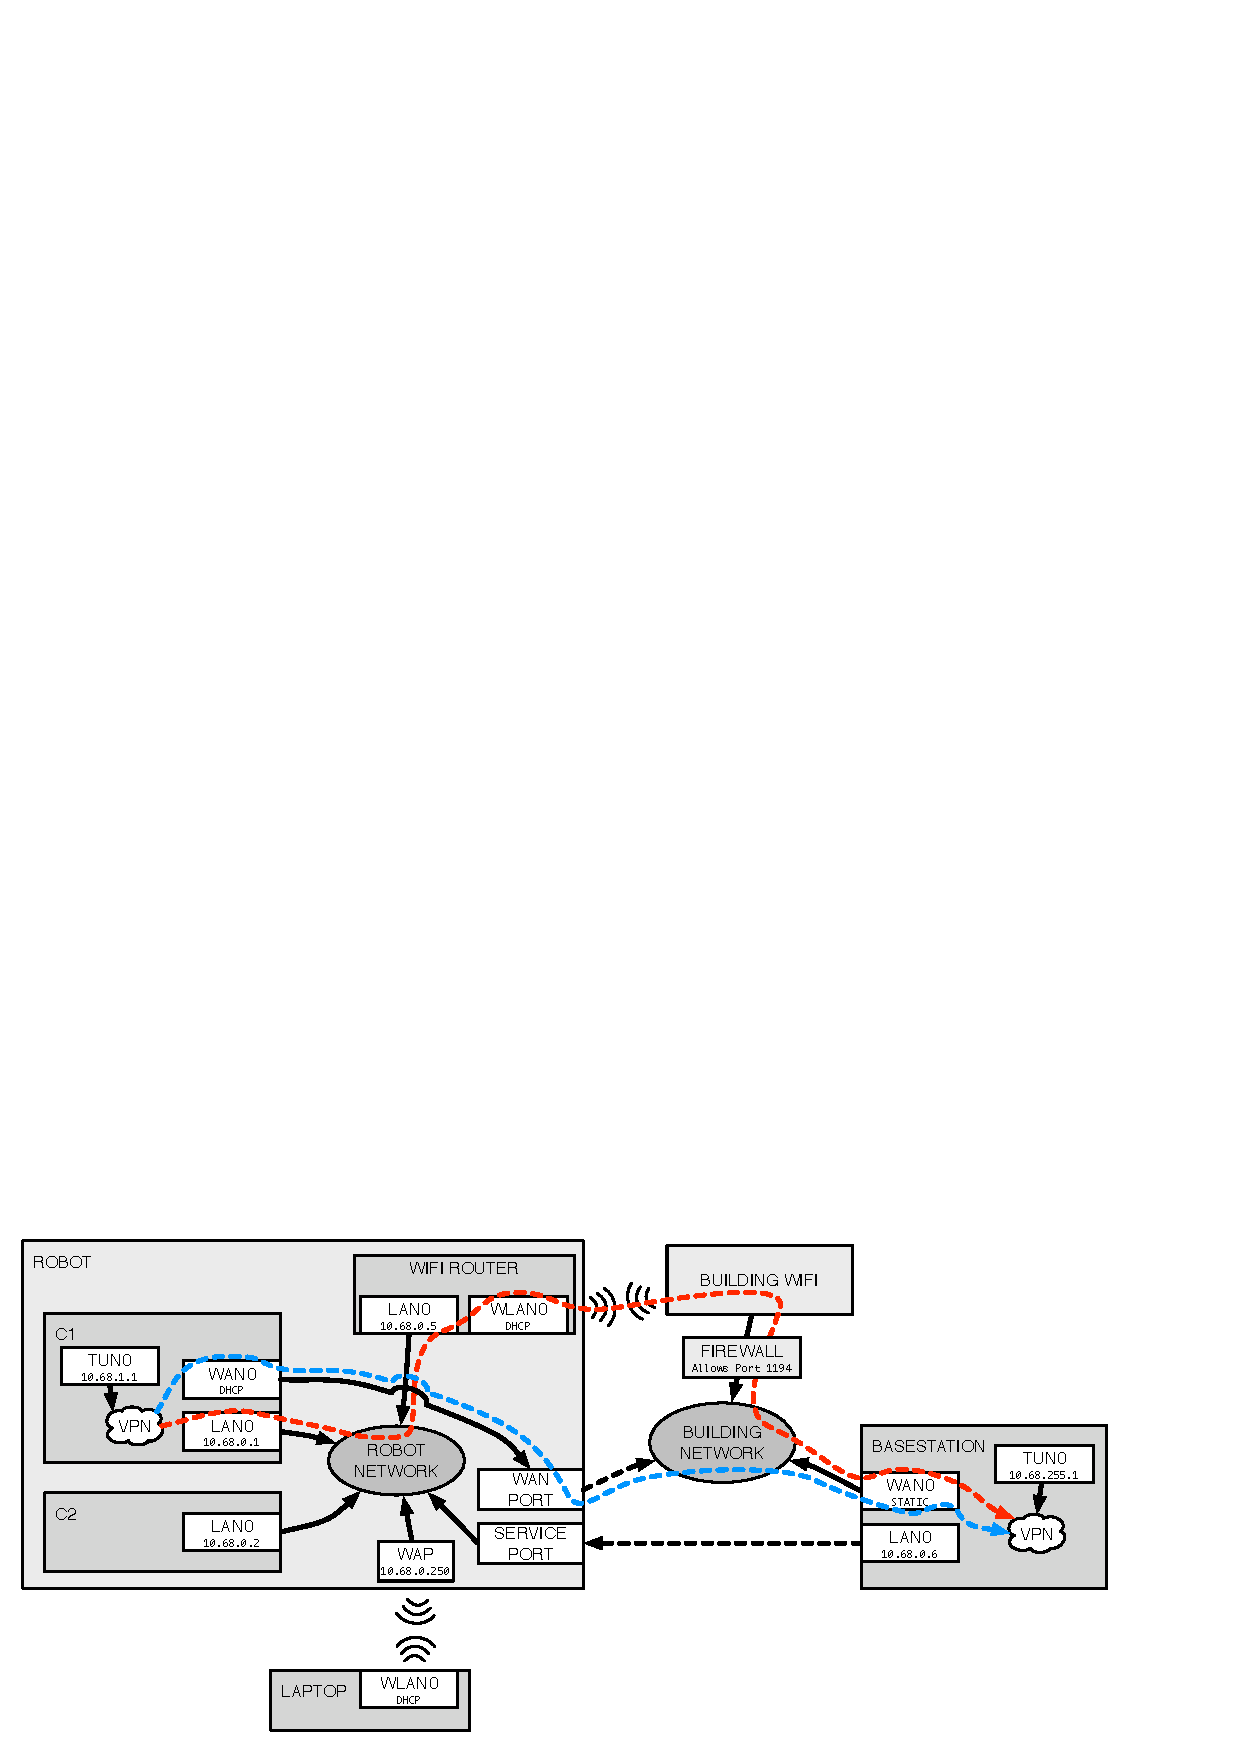
\includegraphics[width=400px]{images/pr2_network_diagram.pdf}

The above figure depicts the interaction between the robot and
building networks.  The dotted lines show paths which may or may not
be connected at any given point in time.  That is, the basestation or
a laptop may not always be plugged into the service port, and the
robot WAN port may not always be plugged into the building network.
The colored lines depict pathways that different network traffic
follows.  The main thing of importance to note is that there are three
ways to talk to the robot: direct wire, direct wireless, or VPN.
Additionally, the VPN traffic itself can be routed in one of two ways,
either via a wired or wireless path.
the VPN.  \textit{Note: for clarity, we have labeled all interfaces
  connected to the building network as WAN, and interfaces connected
  to the robot network as LAN, but this may well not be the case for
  laptops or desktops on your actual network, where the usual default
  interface name is typically ``eth0''}
\begin{itemize}
\item \textbf{Direct wired connection}.  One possibility is to connect
  a laptop, or the basestation \texttt{lan0} port to the robot service
  port.  This simply puts the laptop, or the basetation directly on
  the robot internal network.  The basestation is always configured to
  use the IP address \texttt{10.68.0.6}, whereas the laptop will
  likely be configured to use DHCP.  When plugged into the service
  port, you can talk to the robot LAN ports directly on the
  \texttt{10.68.0.0/24} subnet.  This system will work even if the VPN
  system is not functioning.  This is typically used for reinstalling
  the robot, or debugging other networking problems.
\item \textbf{Direct wireless connection}.  Another possibility is to
  connect a laptop directly to the robot WAP.  This is essentially
  identical to plugging into the service port.  The robot computers
  can be reached directly on the \texttt{10.68.0.0/24} subnet.
\item \textbf{VPN connection}.  When not plugged into the service
  port, the basestation and robot communicate over VPN.  The
  basestation acts as the VPN server, and is always reachable at
  \texttt{10.68.255.1}.  However, there are two mechanism through
  which the VPN traffic may be routed.
  \begin{itemize}
  \item \textbf{Wired VPN connection}. The wired VPN connection is
    depicted in blue.  This only occurs when the robot WAN port is
    plugged into the building network.  Note that \texttt{wan0} on c1
    goes directly to the robot WAN port.  When this is plugged into
    the building network, c1 acquires an IP address via DHCP.  At that
    point c1 initiates a connection to the basestation using a
    specified static IP address.  Once this connection is established,
    all vpn traffic is routed through this pathway.
  \item \textbf{Wireless VPN connection}.  The wireless VPN connection
    is depicted in red.  If the WAN port is not plugged in, the robot
    falls back on its wireless connection.  A secondary route instead
    sends traffic through the wifi-router, which must be configured to
    connect to the building wireless network.  In many cases, the
    wireless network is located outside the firewall, so it is
    important that the static IP of the basestation resolves properly
    and is allowed through the firewall on port 1194.
  \end{itemize}
  Regardless of how the robot is connected to the basestation, a
  desktop situated on the building network will always talk to the
  robot in the same way.  Traffic from the desktop, depicted in green,
  is actually routed through the basestation and into the VPN tunnel.
  Once in the tunnel, which pathway the robot is using is abstracted
  and the traffic seamlessly emerges from the other side of the
  tunnel.
\end{itemize}

\subsection{Service Port} The robot service port is the bottom
ethernet port on the back panel of the robot.  It connects directly to
the robot internel network, allowing you to connect to the computers
directly.  \textit{DO NOT PLUG THIS PORT INTO YOUR BUILDING NETWORK.}
c1 serves DHCP for this network and if it conflicts with another DHCP
server this will most likely cause problems both on your building
network and on the robot network depending on which DHCP server takes
precedence.
\subsection{WAN port} The robot WAN port is the top ethernet port on
the back panel of the robot.  This connects directly to \texttt{wan0}
on c1.  This port is intended to be plugged into your building
network.  The robot will attempt to acquire an IP address via DHCP,
and then attempt to contact the basestation at a known IP address.
\subsection{Wireless access point} The robot comes configured with a
cradlepoint ctr350 configured as a Wireless Access Point (WAP)
\href{http://www.cradlepoint.com/products/ctr350-mobile-broadband-router}.
The ESSID of this network defaults to ``<ROBOTNAME>\_LAN'', and allows
direct access to the Robot Internal Network.  You can configure the
WAP by plugging into the robot service port and going to the IP
address: \texttt{10.68.0.250}.  The default login and password are
``root'', ``willow.''

\subsection{Wireless router}
The PR2 has a
\href{http://www.linksysbycisco.com/US/en/products/WRT610N}{Linksys
  WRT610N} dual-N band wireless router.  This router can be configured
to connect to your building wireless network.  In the absence of a WAN
connection, the robot will attempt to contact the basestation through
this wireless router instead. You can configure the wireless router by
plugging into the robot service port and going to the IP address:
\texttt{10.68.0.5}.  The default login and password are ``root'',
``willow.''

\section{OS}
The operating system running on the PR2 computers is an extended
version of Ubuntu 9.04 (Jaunty Jackalope). It depends on a number of
additional packages for system configuration, but should otherwise be
familiar to for Ubuntu users. If you run into a computer problem not
covered by the PR2 documentation, the
\href{https://help.ubuntu.com/9.04/index.html}{Ubuntu Documentation}
is the next place to look.

\subsection{Networking}
To keep connections behaving sensibly when transitioning the VPN
connection to the basestation, the robot is configured to route ALL
traffic that is not on the robot internal network out through the
basestation.  This means that if VPN is not connected your robot will
not be able to see the outside world even though it might appear that
the network is configured appropriately.

This is handled using an \texttt{ip rule} configuration.  Most of
these rules are added by the init-script:
\texttt{/etc/init.d/iprules.sh}.  If you need to temporarily disable
the rule preventing traffic from going anywhere but the basestation,
you can manually remove the rule:

\begin{verbatim}
pr2admin@c1$ sudo ip rule del priority 3000
\end{verbatim}

This may be useful to do when repairing a system in a particularly bad
state since otherwise you may not be able to fetch necessary software
updates or download necessary configuration files.

\subsection{NFS and Unionfs}
The single largest difference between a normal Ubuntu installation and
the PR2 configuration is that c2 mounts nearly its entire filesystem
via NFS.  The exceptions to this are the directories \texttt{/etc},
\texttt{/var}, and \texttt{/pr2bin} which are mounted via
unionfs-fuse.  In short, unionfs allows one to specify an additional
overlay on top of the underlying filesystem.  The contents of this
overlay can be found in the directory \texttt{/slave} on c1.  Files
added here will show up in the appropriate location on c2.  For more
information on how this is set up, see the man page for
\texttt{unionfs-fuse} and look at the init-script
\texttt{/etc/unionfs-fuse-nfs-root}.

New software and configuration changes should only be made on c1.
Since c2 mounts most of its filesystems read-only, this will usually
be enforced for you.  If you are using a non-standard piece of
software that attempts to write to the filesystem outside of your home
directory you will likely need to make accommodating changes to either
the computer configuration or the software you are trying to run.

\subsection{autofs}
Both of the computers have automount configured for mounting the
\texttt{/home} partition of the other computer in a
computer-independent way using autofs. These automounts are located in
the directory \texttt{/pr}. To get to the home partition on c1 you can
use the path \texttt{/pr/1/} and to get to the home partition on c2
you can use the path \texttt{/pr/2/}. You should rarely need to do
this explicitly, but it is necessary to make sense of home directory
locations.

\subsection{Home directories}
The default configuration for user home directories (as given in
\texttt{/etc/passwd}) is \texttt{/u/username}.  Instead of a
directory, this location is by default a symlink to
\texttt{/pr/1/username} (locating the home directory on c1).  To place
a users home directory at a different location, such as the disk on
c2, an admin can simply move (or copy) the home directory and update
the symlink accordingly.

\subsection{Kernel}
Discuss RT\_PREEMT and anything else non-vanilla about the kernel.
(BLAISE HAS AGREED TO FILL THIS IN).

\subsection{Storage}
Each computer has two hard-drives - one internal 2.5" 500Gb
\href{http://www.seagate.com/www/en-us/products/laptops/momentus/momentus_7200.4_g_force/}{Seagate
  Momentus} drive, and a slot for a removable 3.5" SATA hard-drive
that is exposed on the top of the robot base.

By default the only hard-drive used is the internal drive on c1.
There are 3 relevant partitions created during installation:
\begin{itemize}
\item \texttt{c1:/dev/sda1} -- \texttt{/} -- holds the root filesystem
  for the OS
\item \texttt{c1:/dev/sda5} -- \texttt{c1:/home} -- stores user home
  directories (linked to from \texttt{/u} by way of \texttt{/pr/1})
\item \texttt{c1:/dev/sda6} -- \texttt{/hwlog} -- stores hardware logs
  generated by the pr2
\end{itemize}

The internal hard-drive on c2 has a single partition, which is
generally used as extra user storage:
\begin{itemize}
\item \texttt{c2:/dev/sda1} -- \texttt{c2:/home} -- stores user home
  directories (linked to from \texttt{/u} by way of \texttt{/pr/2})
\end{itemize}

Finally, both computers are configured to conveniently make use of the
additional removable drives.  Any drive loaded into the removable bay
should always show up as \texttt{/dev/removable}.  The mount point:
\texttt{/removable} is set up to allow users to mount the first
partition on this drive.
\begin{itemize}
\item \texttt{/dev/removable1} -- \texttt{/removable} -- stores
  temporary data users may want to move off the robot, primarily used
  for large bag files.  This is NOT mounted by default.  To use a
  driver users must explicitly
\begin{verbatim}
user@c1$ mount /dev/removable
\end{verbatim}
to use it, and should 
\begin{verbatim}
user@c1$ umount /dev/removable
\end{verbatim}
when done.  Until the drive is unmounted, you do not have a guarantee
the data has been written to disk, and if the robot runs out of
batteries, your data may be lost.
\end{itemize}

\subsubsection{Formatting Drives}
If you want to partion / reformat one of the removable drives, or the
the internal drive on c2, you can use the \texttt{formatdisk} helper
utility.  Simply pass it the name of the drive you want to format, for
example:
\begin{verbatim}
pr2admin@c2$ sudo formatdisk /dev/sda
\end{verbatim}
or
\begin{verbatim}
pr2admin@c1$ sudo formatdisk /dev/removable
\end{verbatim}

\subsection{Default user account}
The default account on the robot is ``pr2admin''.  When the robot is
first installed, it does not have a password set, however, this
password is set as part of the branding process.  When you first
receive the PR2 from Willow Garage the password will most likely be
set to ``willow''.

\subsection{Creating user accounts}
The expectation is that each person logging into the robot to develop
code will have their own user account.  Any robot admin can create a
new user using the
\texttt{\href{http://unixhelp.ed.ac.uk/CGI/man-cgi?adduser}{adduser}}
command (NOT the \texttt{useradd} command), on c1.  User accounts are
automatically mirrored on c2.

Some examples:
\begin{verbatim}
pr2admin@c1$ sudo adduser bob
pr2admin@c1$ sudo adduser bill --shell /usr/bin/tcsh --uid 2000
\end{verbatim}

\textit{Note: it may be helpful to assign users the same UID used on
  your building network so the UIDs are consistent when mounting shares
  or moving around the removable drives.}

Moving the home directory and creating the symlink is handled for you
by the script: \texttt{/usr/local/sbin/adduser.local}, which gets run
automatically as a part of user-creation.  You should not need to
worry about this script at all unless you are changing the
user-creation process.

\subsection{User groups}
There are a couple of important groups on the pr2:
\begin{itemize}
\item \texttt{admin} -- Members of this group have full root privileges when using the sudo command
\item \texttt{rosadmin} -- Members of this group have access to change ros-specific configuration settings in \texttt{/etc/ros}
\item \texttt{apt} -- Members of this group can install new software
\end{itemize}

To add a user to a group, use the
\texttt{\href{http://unixhelp.ed.ac.uk/CGI/man-cgi?usermod}{usermod}}
command.  The most common invocation uses the options \texttt{-a}
(append) and \texttt{-G} (group).  For example:

\begin{verbatim}
pr2admin@c1$ sudo usermod -a -G admin bob
\end{verbatim}

\subsection{Backing up and restoring users}
Before reinstalling the robot operating system you will likely want to
back up the user accounts. This can be done with the command:
\texttt{pr2-usermigrate}. To save users:
\begin{verbatim}
pr2admin@c1$ sudo pr2-usermigrate save myrobot.users
\end{verbatim}

Move this file off the robot before reinstalling.  Then, to restore users:
\begin{verbatim}
pr2admin@c1$ sudo pr2-usermigrate load myrobot.users
\end{verbatim}

\subsection{Clock synchronization}
Consistent time-stamping of data from the two computers is important
for interpreting sensor data on a moving system.  As a result, keeping
the system time on the two computers synced together requires some
attention.  The system that is used for this is
\href{http://chrony.tuxfamily.org/}{chrony}, and the general strategy
is to have the two computers tightly coupled to one another, but
loosely coupled to an external time source to prevent the robot time
from drifting too far from the outside world.

If you find your clocks in an inconsistant state, you may want to try
restarting chrony on the basestation, c1, and c2, in that order.
\begin{verbatim}
pr2admin@basestation$ sudo /etc/init.d/chrony restart
pr2admin@c1$ sudo /etc/init.d/chrony restart
pr2admin@c2$ sudo /etc/init.d/chrony restart
\end{verbatim}

\section{Basestation Setup and Pairing}
Before you can use the robot and basestation, it needs to be
configured.  This configuration can be done by logging into the
basestation.  The default account is ``pr2admin'' with password
``willow''.  The following instructions assume that the basestation is
plugged into the robot via the service port.

\subsection{Requirements}

\subsubsection{Naming}
It order for ROS to work properly, it depends on each computer in your
system being able to correctly resolve the hostnames of all other
computers in your ROS system.  For an in depth explanation, please
familiarize yourself with
\href{http://www.ros.org/wiki/ROS/NetworkSetup}{http://www.ros.org/wiki/ROS/NetworkSetup}.
However, in short, you are probably going to need 3 hostnames, and 3
IP addresses -- one for the basestation, and one for each of the two
robot computers.  Each of these 3 hostnames MUST either be resolved by
your building network DNS server, or else they will need to be added
to the \texttt{/etc/hosts} file of all the relevant computers.

\subsubsection{IP Address configuration}
For the robot to be able to find the basestation, it needs to be given
a constant IP address.  Unless you have a reason not to, this IP
address should be assigned to the basestation statically.  However, if
you are certain that your DHCP server will always assign the same IP,
it is ok for this IP to be assigned via DHCP.

The IP address assigned to your basestation must be visible on both
the wired and wireless segments of your building network on port
\texttt{1194}.  This is the port that VPN uses when the robot makes
its connection back to the basestation (it can be changed by modifying
\texttt{/etc/openvpn/server.conf} on the basestation).  Depending on
how secure your network is, and whether these segments are separated
by a firewall, you may need assistance from your local sysadmin to
allow traffic through on this port.

Finally, for the robot to be able to find the basestation, both the
wired and wireless networks must provide a DHCP server.  The operation
of the system is that the robot will acquire an IP address via DHCP
and then contact the basetation at the known IP address that it is
paired to.  Review the section on Networking for a more thorough
overview.

\subsubsection{Examples}

In the remainder of the examples in this section we will assume that
our basestation has been given the hostname \texttt{prbase1}, and our
computers will be named \texttt{prx1} and \texttt{prx2}.  We assume
that DNS resolves them correctly as follows:

\begin{itemize}
\item \texttt{prbase1} -- \texttt{192.168.1.100}
\item \texttt{prx1} -- \texttt{192.168.1.101}
\item \texttt{prx2} -- \texttt{192.168.1.102}
\end{itemize}

\subsection{Plugging things in}
\includegraphics[width=350px]{images/pr2_basestation_plugs.pdf}

When plugging in the basestation, make sure that you plug WAN0 (on the
motherboard) into your building network.  LAN0, on the PCI card, is
only intended to be plugged into the robot service port.

Additionally, it is important to plug the DVI port into the installed
graphics card (on the right side of the computer) and not the extra
DVI port on the motherboard.

There is only one place to plug in the power, and your keyboard/mouse
can be plugged into any of the available USB ports.

\subsection{Configure the Basestation Network}

There are two ways to set up the basestation, using a static IP, or
DHCP.  It is strongly recommended that you use a Static IP unless you
have a very good reason to use DHCP and understand configuring your
DHCP server to obey client-id-based requests.

\subsubsection{Static IP}

To configure the basestation with a static IP, you must edit the file
\texttt{/etc/network/interfaces} and change \texttt{wan0} to use a staic ip
address, for example:
\begin{verbatim}
iface wan0 inet static
      address 192.168.1.100
      netmask 255.255.255.0
      gateway 192.168.1.1
      post-up robot-forward start
      pre-down robot-forward stop
\end{verbatim}
You will also need to update \texttt{/etc/resolv.conf} to contain the
appropriate nameserver, e.g.,
\begin{verbatim}
domain school.edu
search school.edu
nameserver 192.168.1.1
\end{verbatim}

\subsubsection{DHCP}
If you are using DHCP, you must make sure that your DHCP server
respects the client-id specification and is configured to assign a
consistant IP address to the client-id of the basestation.
\textit{NOTE: macaddress based assignment of IPs will not work
  correctly because the basestation also acquires IPs on behalf of the
  robot.}  The default client-id for the basestation is
``basestation.''  If you need to change this to a different client-id,
you must edit the file \texttt{/etc/dhcp3/dhclient.conf}, and change
the relevant line, for example
\begin{verbatim}
send dhcp-client-identifier "prbase1";
\end{verbatim}

\subsubsection{Hostname}
You will also likely need to change the hostname of the basestation.
Leaving it as ``basestation'' is ok, but you need to make sure the DNS
server correctly resolves this name to the IP address you have
assigned the basestation.  To change the hostname you will need to
edit the files: \texttt{/etc/hostname}, to just contain the name of
the basestation.  For example:
\begin{verbatim}
prbase1
\end{verbatim}
and edit \texttt{/etc/hosts} to resolve the basestation locally.
After modifying, \texttt{/etc/hosts} it should look something like:
\begin{verbatim}
127.0.0.1       localhost
127.0.1.1       prbase1.willowgarage.com        prbase1

# The following lines are desirable for IPv6 capable hosts
::1     localhost ip6-localhost ip6-loopback
fe00::0 ip6-localnet
ff00::0 ip6-mcastprefix
ff02::1 ip6-allnodes
ff02::2 ip6-allrouters
ff02::3 ip6-allhosts

### The following lines were added automatically by pr2-basestation ####
10.68.0.1 c1
10.68.0.2 c2
### The preceeding lines were added automatically by pr2-basestation ###
\end{verbatim}
Finally, you need to actually set the hostname using the hostname command, for example:
\begin{verbatim}
pr2admin@basestation$ sudo hostname prbase1
\end{verbatim}

\subsubsection{Applying Settings}
Once you have reconfigured the network, you should reboot the
basestation to make sure the network comes back up correctly.

\subsection{Configure the Robot Wifi}
The Linksys wrt610n on the robot is located at the IP address:
\texttt{10.68.0.5}. To configure it, either plug a laptop or a
basestation into the robot service port, open a web-browser and go to:
\texttt{http://10.68.0.5}.  Click on the ``Wireless'' tab.  The
default login should be ``root'' and ``willow,'' although after a
factory reset the router may end up with login, ``root'' and
``admin''.  Set either ``Wireless Physical Interface wl0'' (for 2.5
Ghz) or ``Wireless Physical Interface wl1'' (for 5 Ghz) to client mode
and enter the SSID for your network.  If you need to change other
settings, make sure that under ``Setup,'' the WAN connection type is
``Automatic Configuration - DHCP'', the local IP Address is
\texttt{10.68.0.5}, and the DHCP Server is Disabled.  When you are
done, make sure you choose to ``Apply Settings.''

To test the setup of the wireless, you can temporarily add a route on
the basestation which will route a particular IP address through the
wifi router.
\begin{verbatim}
$ sudo ip route add 157.22.19.22 via 10.68.0.5 dev lan0
\end{verbatim}
Then point your web-browser to: \texttt{http://157.22.19.22}. This
should take you to the willowgarage home page.  

It may take a short time for the wireless router to connect to the
network. 

Once that is working, you should remember to disable the route so that
it works if the basestation is not plugged into the service port:
\begin{verbatim}
$ sudo ip route del 157.22.19.22 via 10.68.0.5 dev lan0
\end{verbatim}

\subsection{Initialize the Basestation VPN Server}
One of the primary functions of the basestation is to host a VPN
server that the robot can connect to.  The server needs an appropriate
key.  To generate the key for the VPN server run:

\begin{verbatim}
pr2admin@basestation$ sudo /etc/openvpn/gen_server_key
\end{verbatim}

It will prompt you for some information.  It is good practice to get
the information correct, but will not actually impact the performance
of the robot.

\subsection{Pairing with the Robot}

Robot pairing is performed with the the \texttt{robot-brand} command
on the basestation.  It takes 5 arguments:

\begin{itemize}
\item robotname -- This is the name your robot will be given.
\item c1name -- This is the intended hostname of c1.  Your DNS server needs to resolve this to the IP address you intend to use for your robot.
\item c2name -- This is the intended hostname of c2.  Your DNS server needs to resolve this to the IP address you intend to use for your robot.
\item VPN subnet -- Unless you are using multiple robots, this should be 10.68.1.0.  The 3rd field of the IP, however, can be any value other than 0 and 255, which are reserved for the robot local network and the basestation server respectively.  No two robots on the same basestation should be assigned the same VPN subnet.
\item Basestation IP -- This is the static IP address you have assigned to your basestation \texttt{wan0}.
  It is worth checking that it is correct using the \texttt{ifconfig} command:
\begin{verbatim}
pr2admin@basestation:~$ ifconfig wan0
wan0      Link encap:Ethernet  HWaddr 00:30:1b:48:c8:f8  
          inet addr:192.168.1.100  Bcast:192.168.1.255  Mask:255.255.255.0
          inet6 addr: fe80::230:1bff:fe48:c8f8/64 Scope:Link
          UP BROADCAST RUNNING MULTICAST  MTU:1500  Metric:1
          RX packets:2702 errors:0 dropped:0 overruns:0 frame:0
          TX packets:2709 errors:0 dropped:0 overruns:0 carrier:0
          collisions:0 txqueuelen:1000 
          RX bytes:129699 (129.6 KB)  TX bytes:218528 (218.5 KB)
          Interrupt:17 
\end{verbatim}
In this case the address is \texttt{192.168.1.100}.
\end{itemize}

To actually brand the robot, first plug the basestation into the
service port of the robot, and then use the robot-brand command

\begin{verbatim}
pr2admin@basestation$ sudo robot-brand <ROBOT_NAME> <C1_NAME> <C2_NAME> <VPN_SUBNET> <BASESTATION_IP>
\end{verbatim}

For example, if your robot were going to be named ``prx'', c1 was
going to named ``prx1'', c2 was going to be named ``prx2'', and your
basestation was located at \texttt{192.168.1.100}, you would run:

\begin{verbatim}
pr2admin@prbase1$ sudo robot-brand prx prx1 prx2 10.68.1.0 192.168.1.100
\end{verbatim}

During the branding process, it may prompt you for the password of
``root@c1''.  By default this will be ``willow''.  Additionally, you
may be prompted to choose a password for the pr2admin account.

When the script finishes, you should be able to connect to the robot
over the VPN.  Check that it works and then exit.
\begin{verbatim}
pr2admin@prbase1$ ssh pr2admin@10.68.1.1
pr2admin@prx1:~$ exit
\end{verbatim}

\subsection{Forwarding IPs to the robot}

To make contacting the robot from your building network more convenient,
the basestation can be configured to forward IP addresses (assigned
statically or via DHCP) to the robot.

To set this up, edit the file: \texttt{/etc/robot-forward.conf} and add the lines:

\begin{verbatim}
<C1_NAME> <VPN_SUBNET>.1 <ROBOT_IP1>
<C2_NAME> <VPN_SUBNET>.2 <ROBOT_IP2>
\end{verbatim}

For example, in our case we would use:

\begin{verbatim}
prx1 10.68.1.1 192.168.1.101
prx2 10.68.1.2 192.168.1.102
\end{verbatim}

Note that for this to work properly, we should have named our robot
computers prx1 and prx2, respectively, and furthermore our DNS server
should resolve ``prx1'' to \texttt{192.168.1.101}, and ``prx2'' to
\texttt{192.168.1.102}.

Much like the basestation, you can also have these IPs assigned via DHCP:

\begin{verbatim}
prx1 10.68.1.1 dhcp
prx2 10.68.1.2 dhcp
\end{verbatim}

In which case the basestation will use the client-id's ``prx1'' and
``prx2'' to acquire 2 IP addresses from the DHCP server.  These IPs
should be assigned consistantly given the client-id's, and should
match the IPs that the DNS server returns for the particular hostnames.  

Robot forwarding is enabled whenever the networking starts, but to
manually start forwarding, you can run:

\begin{verbatim}
pr2admin@prbase1$ sudo robot-forward start
\end{verbatim}

You should not be able to contact the robot at the IP address you have
given it, and, if your DNS server is set up properly, using it's
hostname.  For example:

\begin{verbatim}
pr2admin@prbase1$ ssh pr2admin@192.168.1.101
\end{verbatim}

and

\begin{verbatim}
pr2admin@prbase1$ ssh pr2admin@prx1
\end{verbatim}

If you need to disable forwarding you can run:

\begin{verbatim}
pr2admin@prbase1$ sudo robot-forward stop
\end{verbatim}

\section{Software Maintenance}

When the robots ship, the most recent version of ROS and the PR2
software stacks is installed in /opt/ros.  By default, new users will
have a ROS installation which references the pre-installed code.
Users who wish to modify or replace a part of the system are
recommended to install a development version of the stacks or packages
which they wish to modify, but to continue to use the base
installation for most of the robot functionality.

Debian packages exist for all of the custom software and
configurations on the robot.  The package which pulls in all the other
requirements is called \texttt{pr2-environment}.
\texttt{pr2-environment} depends on \texttt{pr2-core}, which in turn
depends on \texttt{ros-boxturtle-pr2}, the meta-package which contains
all of the ROS software for the PR2.

To upgrade the software on your robot, you can simply use \texttt{apt}:

\begin{verbatim}
$ sudo apt-get dist-upgrade
\end{verbatim}

Which will update all packages on your system, pulling in security fixes for
the pr2 configuration as well as for the appropriate ros-release.

\section{Reinstall the Basestation}
If you have a basestation USB installer, you can reinstall the
basestation to revert it to a completely fresh state.  Creating a new
USB installer is outside the scope of this manual, but instructions
for downloading and creating one can be found on the PR2 website.

\subsection{Booting off the USB installer}
To boot off the USB installer:
\begin{itemize}
\item Insert the USB stick into one of the USB ports in the basestation
\item Reboot the basestation
\item Press the \texttt{<DEL>} key to enter setup
\item Choose ``Advanced BIOS Features''
\item Choose ``Hard Disk Boot Priority''
\item Select the drive listed as ``USB-HDD0'' and hit ``Page Up'' to make it number 1
\item Hit ``F10'' to save and exit the setup
\item The computer should boot off of the USB stick.
\item If the installer complains about not being able to find the ISO, hit ``Enter'' to continue, twice and the installation should continue.
\item When the installer completes, hit ``Enter'' to shut down and remove the USB stick.
\item When the basestation boots you should have a fresh image -- consult the section on Basestation Setup and Pairing to configure the basestation.
\end{itemize}

\section{Reinstall the Robot}

To reinstall the robot, first back up anything you need off of c1.
Next, shutdown the comptuers using \texttt{pr2-shutdown --netboot}.

You must then plug the service port directly into the basestation.
You can then run the robot installer:

\begin{verbatim}
pr2admin@basestation$ sudo robot-install
\end{verbatim}

Boot c1 by pushing the power button with a paperclip.

After N minutes, the netconsole on the basestation will show the
install dialog.  Hit enter to start the installer and wait for it to
complete.

Once the installer has completed and the robot is shut down, you can
boot it up.  You will now need to pair it with the basestation before
you can use it.

\subsection{Forcing netboot}

If the robot BIOS is not configured to netboot, you might need to be
able hit f12 on the keyboard.  You can do this in one of two ways.

The easier way to to connect up to the KVM.  (See section XYZ on connecting to the KVM.)

Alternatively, plug a keyboard into the PR2.  This can be done using
the aux usb port under the back cover.  To remove this cover, follow
the instructions in section XYZ.

When the robot is booting you will hear 2 beeps followed by a short
pause, and then another 2 beeps.  After the 4th beep, hit f12 on the
keyboard (either physically or through the KVM) to force c1 to netboot.


\chapter{Software on PR2}
\section{pr2\_core}
There is a core set of code that always runs by default on the robot.  This includes:
\begin{description}
\item[roscore]
\item[diagnostics logging] to /hwlogs
\item[web interface] which exports a set of webpages at XXX for basic robot control
\item[pr2\_etherCAT]
\item[power\_board]
\item[battery\_monitor]
\item[sensor drivers]
This list is controlled by the launch files in XXX, which are used by rosinit on startup, and any time that the robot needs to "reset" to the default state (or when a developer wants to change one of those components)
\end{description} 
\section{pr2\_dashboard}
pr2\_dashboard, Figure~\ref{fig:dashboard}, is a GUI for debugging and controlling low-level state of the PR2. The dashboard displays the diagnostic, 
circuit breaker, runstop, and battery status.
\begin{figure}[h]
\centering
\includegraphics[scale=0.5]{pr2_dashboard.png}
\caption{The PR2 dasboard.}
\label{fig:dashboard}
\end{figure}
\begin{description}
\item[Diagnostic Status] The state of the robot is shown by the diagnoctic indicators in the pr2\_dashboard. \\

    \newcolumntype{S}{>{\centering\arraybackslash} m{.9cm} }%
    \begin{tabular}{m{6cm}SSSS}
    Component & OK & Warn & Error & Stale\\
    &&&&\\
    Diagnostics: Clicking pops up the Robot Monitor & \includegraphics[scale=0.5]{diag_error.png}&\includegraphics[scale=0.5]{diag_warn.png}&
                                                      \includegraphics[scale=0.5]{diag_ok.png}&\includegraphics[scale=0.5]{diag_stale.png}\\
    &&&&\\
    Rosout: Clicking pops up rxconsole & \includegraphics[scale=0.5]{rosout_error.png}&\includegraphics[scale=0.5]{rosout_warn.png}&
                                        \includegraphics[scale=0.5]{rosout_ok.png}&\includegraphics[scale=0.5]{rosout_stale.png}\\
    &&&&\\
    Motors: Clicking allows you to halt or reset motors & \includegraphics[scale=0.5]{motor_error.png}& N/A &
                                                          \includegraphics[scale=0.5]{motor_ok.png}&\includegraphics[scale=0.5]{motor_stale.png}\\
   \end{tabular}

\item[Circuit Breaker Status] The circuit breakers are labeled L/B/R, which stand for Left Arm, Base/Spine, and Right Arm. 
Each breaker can be in one of four states, and clicking on any of the breakers will pop up a menu, Figure~\ref{fig:breaker_menu}, allowing you to change 
the state of one or all of them:
\begin{figure}[h]
\centering
\includegraphics[scale=0.5]{breakers_menu.png}
\caption{The circuit breaker options menu.}
\label{fig:breaker_menu}
\end{figure}

    \newcolumntype{S}{>{\centering\arraybackslash} m{1.7cm} }%       
    \begin{tabular}{m{2.6cm}SSSS}
     & Enabled & Standby & Disabled & Stale\\
    Breaker Status & \includegraphics[scale=0.5]{L_ok.png}\includegraphics[scale=0.5]{B_ok.png}\includegraphics[scale=0.5]{R_ok.png}&
                     \includegraphics[scale=0.5]{L_stby.png}\includegraphics[scale=0.5]{B_stby.png}\includegraphics[scale=0.5]{R_stby.png}&
                     \includegraphics[scale=0.5]{L_dis.png}\includegraphics[scale=0.5]{B_dis.png}\includegraphics[scale=0.5]{R_dis.png}&
                     \includegraphics[scale=0.5]{L_stale.png}\includegraphics[scale=0.5]{B_stale.png}\includegraphics[scale=0.5]{R_stale.png}\\
   \end{tabular}



\item[Runstop Status] The runstop indicators display the staus of the PR2 runstops and their state cannot be changed using the dashboard. 
There are two runstops on the robot, a wireless runstop, see \ref{wirelessrunstop}, and a physical runstop on the back of the robot.

\item[Battery Status]

\end{description}

\section{Apps}
This section should contain a list of all the top-level useful apps shipping with the PR2.  We need some template for structuring this data, and ideally this documentation would be pulled from the apps themselves.

\subsection{joystick\_teleop or replacement}
\subsection{...}
\section{Data and robot configuration}
\subsection{Robot description}
\subsection{pr2.launch and pr2.urdf}
Local versions of launch file and urdf that live in /etc/pr2/ and can be calibrated, changed to accomodate new sensors or robot changes, etc.

Describe API of full robot here (what topics, services, etc. the PR2 has when it's up)
\subsubsection{Integrating calibration data}
Basically, over-write /etc/pr2/pr2.launch

\chapter{Writing code on PR2}
The PR2 comes with the PR2 varient of the latest released distribution
or ROS installed from binary debian packages in \texttt{/opt/ros} .  It is
recommended to use this installation for it saves compile time and
disk space.
\section{Installing code in user-space}
To setup your environment with the installed packages type:
\begin{verbatim}
. /opt/ros/boxturtle/setup.sh
\end{verbatim}
\subsection{Installing another repository in user-space}
To add another repository an overlay rosinstall file should be created
like the following:
\begin{verbatim}


\end{verbatim}

Then type:
\begin{verbatim}
~/rosinstall -o ~/local_dir ~/custom.rosinstall
\end{verbatim}
\subsubsection{Setting environment to use local\_dir}
\begin{verbatim}
. ~/local_dir/setup.sh
\end{verbatim}

\subsection{Creating a package}
This is documented on the wiki in the
\href{http://www.ros.org/wiki/roscreate}{roscreate package}

\subsection{Using a local version of a stack}
If a different version of a stack is desired instead of an installed
one, add it to your overlay rosinstall file.  Stacks in overlays are
prepended to the path and thus will take priority over an existing
stack.  Note be careful, if changing a lower level stack, for all
things which depend on it's changes must be rebuilt. This can be an
issue if the dependent stacks are also installed.

\section{Where to Start}
\subsection{Documetation and Tutorials}
Documentation for ROS and the PR2 can be found on \href{http://www.ros.org}{ros.org}. An overview 
of the relevant libraries for filtering, navigation, cooridinate tranforms, etc., can be foung at 
\href{http://www.ros.org/APIs}{http://www.ros.org/APIs}. Below is a listing of several tutorials 
for learning and using ROS:
\begin{description}
\item[\href{http://www.ros.org/wiki/ROS/Tutorials}{ROS stack tutorials}] These tutorials cover the
basic ROS concepts and tools for writing and using ROS nodes.
\item[\href{http://www.ros.org/wiki/tf/Tutorials}{tf tutorials}] These tutorials cover using the tf 
library for cooridinate transofrms using the python and C++ APIs.
\item[\href{http://www.ros.org/wiki/navigation/Tutorials}{navigation tutorials}] These tutorials 
cover configuring and using the navigation stack on the PR2 and other robots.
\item[\href{http://www.ros.org/wiki/laser_pipeline/Tutorials}{laser\_pipeline tutorials}] These tutorials 
cover processing laser data and converting laser data into 3D representations.
\item[\href{http://www.ros.org/wiki/image_common/Tutorials}{image\_common tutorials}] These tutorials 
cover working with images in ROS.
\item[\href{http://www.ros.org/wiki/actionlib_tutorials/Tutorials}{actionlib tutorials}] These 
tutorials cover implementing actions, a standard interface preemptible highlevel tasks, using 
the python and C++ APIs. More example tutorials can be found at 
\href{http://www.ros.org/wiki/turtle_actionlib}{turtle actionlib}.
\end{description}

\subsection{Mailing Lists}
\begin{description}
\item[\href{https://lists.sourceforge.net/lists/listinfo/ros-users}{ros-users}] This mailing list 
provides the latest ROS news and is a forum for posting questions to the ROS community for help. 
\item[\href{http://lists.willowgarage.com/cgi-bin/mailman/listinfo/pr2-users}{PR2-users}] This 
mailing list provides the latest PR2 news and is a forum for posting questions to the PR2 community 
for help.
\end{description}



\chapter{Maintaining PR2}
\section{Installing upgraded stacks}
Instructions on using the pr2\_admin user to install new version of stacks and apps next to what is already on the system.

Instructions on how users set up their accounts to be either using the latest code all the time or to be locked to a particular version.  Discussion of the advantages of each.
\section{Installing updated disk images}
Instructions on installing an updated disk image from WG on the PR2 for, e.g. OS changes or robot configuration updates.  We need to figure out what is maintained during updates (e.g. network configuration?), and what is over-written.  This needs to be crisp and well-documented.
\section{Resetting PR2}
Sometimes, you may want to reset PR2 to factory defaults.  This is the process.
This can either be done while preserving user data, or can be done as a full factory reset.

Essentially, this is a full update to the last-installed disk image.
\section{Diagnostics Logs}
Since the PR2 is currently in beta, it is important for us to learn as much as we can about robot hardware usage and how problems develop.  To address this, we are requiring all PR2 beta sites to regularly transfer diagnostics logs to Willow Garage.

These logs are gathered automatically by pr2\_core in the /hwlogs partition.  This directory should not be used for anything else, since everything there will be periodically transfered to Willow Garage.
\subsection{Setting up automatic transfer}
To make this process easier, we have provided a set of scripts to perform this log transfer automatically.  To enable those, just add the line XXX to the pr2\_admin crontab via these instructions:
\subsection{Manual transfer}
If you would prefer to not have the robot transfer logs back to Willow Garage automatically, you can transfer them manually instead.  To do this, either run the script "transfer\_logs", or look inside it to understand what it's doing and perform the transfer yourself.
\section{Solving hardware problems}
\subsection{Figuring out what's wrong}
The first step if you suspect hardware problems should be to check the diagnostics display in pr2\_dashboard.  If that doesn't help you resolve the problem, you can run the full robot self test.  This is a GUI which allows you to select the portions of the robot you wish to qualify, and runs them through a variety of tests to diagnose problems.  Instructions on using it and interpreting the data it outputs go here.
\subsection{Support}
For hardware issues, please submit a ticket at support.willowgarage.com
\subsection{Documentation}
For more detailed documentation, see support.willowgarage.com.  This includes drawings and step-by-step instructions for replacing all user-servicable parts.

After this list of chapters, we should have a set of other tutorials which have been referenced from the text.  Only tutorials that are on the critical path should be in-lined in the text.  Everything else should be referenced and then collected at the end.

\end{document}
